\documentclass{article}

% packages
  % basic stuff for rendering math
  \usepackage[letterpaper, top=1in, bottom=1in, left=1in, right=1in]{geometry}
  \usepackage[utf8]{inputenc}
  \usepackage[english]{babel}
  \usepackage{amsmath} 
  \usepackage{amssymb}
  % \usepackage{amsthm}

  % extra math symbols and utilities
  \usepackage{mathtools}        % for extra stuff like \coloneqq
  \usepackage{mathrsfs}         % for extra stuff like \mathsrc{}
  \usepackage{centernot}        % for the centernot arrow 
  \usepackage{bm}               % for better boldsymbol/mathbf 
  \usepackage{enumitem}         % better control over enumerate, itemize
  \usepackage{hyperref}         % for hypertext linking
  \usepackage{fancyvrb}          % for better verbatim environments
  \usepackage{newverbs}         % for texttt{}
  \usepackage{xcolor}           % for colored text 
  \usepackage{listings}         % to include code
  \usepackage{lstautogobble}    % helper package for code
  \usepackage{parcolumns}       % for side by side columns for two column code
  

  % page layout
  \usepackage{fancyhdr}         % for headers and footers 
  \usepackage{lastpage}         % to include last page number in footer 
  \usepackage{parskip}          % for no indentation and space between paragraphs    
  \usepackage[T1]{fontenc}      % to include \textbackslash
  \usepackage{footnote}
  \usepackage{etoolbox}

  % for custom environments
  \usepackage{tcolorbox}        % for better colored boxes in custom environments
  \tcbuselibrary{breakable}     % to allow tcolorboxes to break across pages

  % figures
  \usepackage{pgfplots}
  \pgfplotsset{compat=1.18}
  \usepackage{float}            % for [H] figure placement
  \usepackage{tikz}
  \usepackage{tikz-cd}
  \usepackage{circuitikz}
  \usetikzlibrary{arrows}
  \usetikzlibrary{positioning}
  \usetikzlibrary{calc}
  \usepackage{graphicx}
  \usepackage{caption} 
  \usepackage{subcaption}
  \captionsetup{font=small}

  % for tabular stuff 
  \usepackage{dcolumn}

  \usepackage[nottoc]{tocbibind}
  \pdfsuppresswarningpagegroup=1
  \hfuzz=5.002pt                % ignore overfull hbox badness warnings below this limit

% Custom Environments
  \newtcolorbox[auto counter, number within=section]{example}[1][]
  {
    colframe = orange!25,
    colback  = orange!10,
    coltitle = orange!20!black,  
    breakable, 
    title = \textbf{Question \thetcbcounter ~(#1)}
  }
  \newtcolorbox[auto counter, number within=section]{definition}[1][]
  {
    colframe = yellow!25,
    colback  = yellow!10,
    coltitle = yellow!20!black,  
    breakable, 
    title = \textbf{Definition \thetcbcounter ~(#1)}
  } 
  \newtcolorbox[auto counter, number within=section]{society}[1][]
  {
    colframe = yellow!25,
    colback  = yellow!10,
    coltitle = yellow!20!black,  
    breakable, 
    title = \textbf{Society \thetcbcounter}
  }
  \newtcolorbox[auto counter, number within=section]{politics}[1][]
  {
    colframe = red!25,
    colback  = red!10,
    coltitle = red!20!black,  
    breakable, 
    title = \textbf{Politics \thetcbcounter ~(#1)}
  }
  \newtcolorbox[auto counter, number within=section]{legal}[1][]
  {
    colframe = blue!25,
    colback  = blue!10,
    coltitle = blue!20!black,  
    breakable, 
    title = \textbf{Legal \thetcbcounter ~(#1)}
  } 
  \newtcolorbox[auto counter, number within=section]{finance}[1][]
  {
    colframe = green!25,
    colback  = green!10,
    coltitle = green!20!black,  
    breakable, 
    title = \textbf{Finance \thetcbcounter ~(#1)}
  } 
  \newtcolorbox[auto counter, number within=section]{religion}[1][]
  {
    colframe = violet!25,
    colback  = violet!10,
    coltitle = violet!20!black,  
    breakable, 
    title = \textbf{Religion \thetcbcounter ~(#1)}
  }
  \newtcolorbox[auto counter, number within=section]{technology}[1][]
  {
    colframe = violet!25,
    colback  = violet!10,
    coltitle = violet!20!black,  
    breakable, 
    title = \textbf{Technology \thetcbcounter ~(#1)}
  }

  \BeforeBeginEnvironment{example}{\savenotes}
  \AfterEndEnvironment{example}{\spewnotes}
  \BeforeBeginEnvironment{lemma}{\savenotes}
  \AfterEndEnvironment{lemma}{\spewnotes}
  \BeforeBeginEnvironment{theorem}{\savenotes}
  \AfterEndEnvironment{theorem}{\spewnotes}
  \BeforeBeginEnvironment{corollary}{\savenotes}
  \AfterEndEnvironment{corollary}{\spewnotes}
  \BeforeBeginEnvironment{proposition}{\savenotes}
  \AfterEndEnvironment{proposition}{\spewnotes}
  \BeforeBeginEnvironment{definition}{\savenotes}
  \AfterEndEnvironment{definition}{\spewnotes}
  \BeforeBeginEnvironment{exercise}{\savenotes}
  \AfterEndEnvironment{exercise}{\spewnotes}
  \BeforeBeginEnvironment{proof}{\savenotes}
  \AfterEndEnvironment{proof}{\spewnotes}
  \BeforeBeginEnvironment{solution}{\savenotes}
  \AfterEndEnvironment{solution}{\spewnotes}
  \BeforeBeginEnvironment{question}{\savenotes}
  \AfterEndEnvironment{question}{\spewnotes}
  \BeforeBeginEnvironment{code}{\savenotes}
  \AfterEndEnvironment{code}{\spewnotes}

  \definecolor{dkgreen}{rgb}{0,0.6,0}
  \definecolor{gray}{rgb}{0.5,0.5,0.5}
  \definecolor{mauve}{rgb}{0.58,0,0.82}
  \definecolor{lightgray}{gray}{0.93}

  % default options for listings (for code)
  \lstset{
    autogobble,
    frame=ltbr,
    language=C,                           % the language of the code
    aboveskip=3mm,
    belowskip=3mm,
    showstringspaces=false,
    columns=fullflexible,
    keepspaces=true,
    basicstyle={\small\ttfamily},
    numbers=left,
    firstnumber=1,                        % start line number at 1
    numberstyle=\tiny\color{gray},
    keywordstyle=\color{blue},
    commentstyle=\color{dkgreen},
    stringstyle=\color{mauve},
    backgroundcolor=\color{lightgray}, 
    breaklines=true,                      % break lines
    breakatwhitespace=true,
    tabsize=3, 
    xleftmargin=2em, 
    framexleftmargin=1.5em, 
    stepnumber=1
  }

% Page style
  \pagestyle{fancy}
  \fancyhead[L]{Postmodern History}
  \fancyhead[C]{Muchang Bahng}
  \fancyhead[R]{Spring 2024} 
  \fancyfoot[C]{\thepage / \pageref{LastPage}}
  \renewcommand{\footrulewidth}{0.4pt}          % the footer line should be 0.4pt wide
  \renewcommand{\thispagestyle}[1]{}  % needed to include headers in title page

\begin{document}

\title{Postmodern History}
\author{Muchang Bahng}
\date{Spring 2024}

\maketitle
\tableofcontents
\pagebreak


\section{1987 Black Monday}

  During a strong 5-year bull market, the DJIA rose from 776 to 2,722. Some causes may have been:  
  \begin{enumerate}
    \item belief that stocks were overvalued and were certain to undergo a correction. 
    \item persistent US trade and budget deficits, leading to a weakening of the US dollar. 
    \item Rising interest rates, making debt more expensive and reducing monetary circulation. 
  \end{enumerate}

\section{1992 Black Wednesday}

  George Soros shorting the British pound. 

\section{2000 Dot-Com Bubble}

  Burst in March 2000. 

\section{2001 Enron Scandal}

  Enron was an American energy, commodities, and services company founded in Houston, Texas in 1985, with Kenneth Lay becoming Enron's CEO and chair. Deregulation of the energy markets allowed companies to place bets on future prices, so Lay created Enron Finance and appointed Jeffrey Skilling, to head the new corporation. 

  Skilling transitioned Enron's accounting practices from a traditional \textbf{historical cost} (you report the value of assets as the price you bought it for) to a \textbf{mark-to-market (MTM)} (you can report it as the current market price).\footnote{This was a legitimate and widely-used practice.} Since MTM measures the fair value of accounts that can change over time and is therefore harder to pin down, this can be manipulated. 

  With these inflated returns, Enron's stock soared (which didn't raise eyebrows since we were in the dot-com bubble anyway), and Enron expanded into a new markets. 
  \begin{enumerate}
    \item During the 1990s, Enron created \textit{EnronOnline}, which was an electronic trading website that focused on commodities, and the firm would be the counterparty to every transaction. Enron was essentially a natural gas market maker. 
    \item In 2000, it partnered with Blockbuster to enter the video-on-demand (VOD) market, which was a sensible pick, but Enron started logging expected earnings based on the estimated growth on the market, vastly inflating the numbers. 
    \item In the same year, Enron decided to build high-speed broadband telecom networks.  
  \end{enumerate}
  These were relatively young and volatile markets, and when the recession hit in 2000, Enron had significant exposure to these markets and took a big hit. 

  To hide the losses, both Skilling and the CFO Andrew Fastow, promoted in 1998, decided to create a network of sister companies, called \textbf{special purpose vehicle (SPV)} to hide Enron's losses.\footnote{SPVs are used strategically to hedge losses by transferring risk to these companies. The problem was that Enron was on both sides of the trade and knew that the SPV was going to fail.} 
  \begin{enumerate}
    \item These independent SPVs would go to banks to receive a loan, using the fact that they are backed by Enron. 
    \item The SPVs would buy Enron stock with cash or a note. 
    \item With the stock, the SPV would hedge an asset listed on Enron's balance sheet, effectively replacing risky assets or losses with cash/income. 
  \end{enumerate}
  Obviously, this sounds very fishy, but Enron, not revealing these conflicts of interest, got away with this. The other big corrupt player was Enron's accounting firm, Arthur Anderson LLP, and partner David B. Duncan, who determined that these standards were acceptable. Soon enough, analysts began to downgrade their rating for Enron's stock, and it descended to a 52-week low, though it was not enough to attract big attention. 

  By October 2001, the company couldn't keep this up and reported its first loss whilst closing it first SPV. This caught the attention of the SEC, leading to an investigation. Fastow was fired, Enron had losses of \$591 million (and \$690 million in debt), and its merger with Dynergy was canceled. By December 2001, Enron filed for bankruptcy. It liquidated assets, paying over \$21.8 billion to investors until 2012. 


\section{2008 Housing Crisis}

  At this point, we must first point out a (faulty) assumption that everybody had on the housing market, which was that \textit{housing prices must keep going up}. This made sense because in more stable times, the supply of land is fixed. This is represented with historical statistics. 
  
  \begin{figure}[H]
    \centering 
    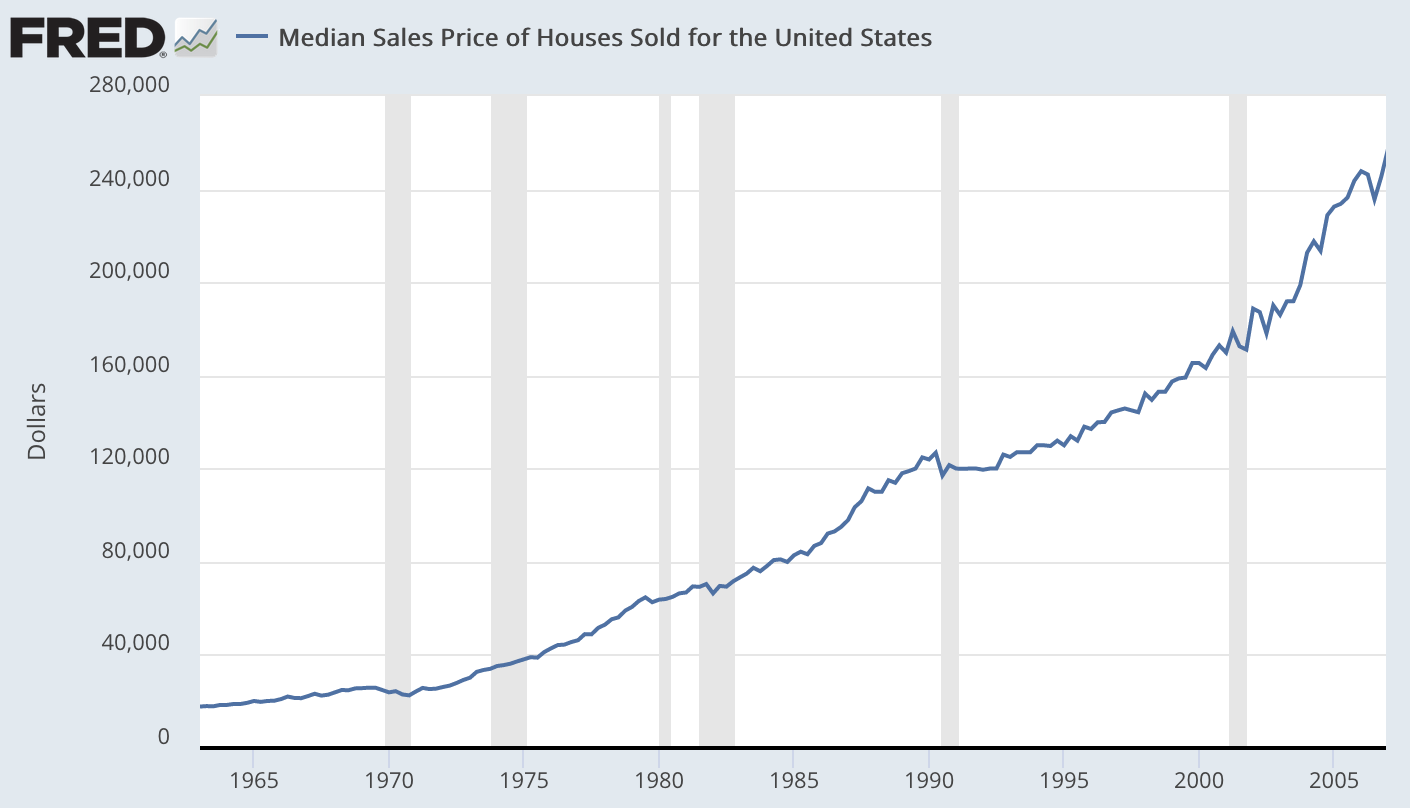
\includegraphics[scale=0.4]{img/housing.png}
    \caption{Housing prices have consistently gone up. From looking at this chart, it's hard to believe that house prices are doing to take a turn for the worse all of a sudden. } 
    \label{fig:housing}
  \end{figure}

  To give some context, after the tech bubble, nobody wanted to lend to tech companies, leading to a dearth in credit. This was worsened through the 9/11 attacks causing uncertainty in the markets. Therefore, to bring back the credit market, the Fed restricted the FFR interest rate from $6.5\%$ in May 2000 to $1\%$ in June 2003. The aim was to incentivize lenders to lend out money and as a result boost the economy by making money available to businesses and consumers at bargain rates. Let's consider the impact that this had on mortgage creditors. With interest rates at an all time low, many borrowers entered into mortgage loans to buy homes. With everybody wanting to buy homes, the household prices kept rising. 

  At this point the lenders, which were commercial banks or lending companies, were impatient and wanted more profits. It turned out that investment banks wanted to buy up these loans (which were not tradable and therefore not securities) and securitize them into something called \textbf{mortgage backed securities (MBS)}. Therefore, lenders would loan out as much mortgages as possible and sell the debt forward to the investment banks for a fee, pocketing a small but easy profit. Doing this hundreds of thousands of times made them lots of money with no risk. The investment banks saw this also as a good investment since these debts were from creditworthy borrowers, and even if they defaulted, the loans were \textit{collaterized}, meaning that they can take the house as collateral. And since house prices are always going up, this was not a problem to the investment banks. Therefore, they would go to a credit rating agency like Moody, S\&P, or Fitch, get an investment grade rating (AAA, AA, or A) with these prime (creditworthy) loans, and sell billions of dollars worth of them to institutional investors who managed things like retirement portfolios, pension funds, or mutual funds.\footnote{Securities must be rated investment grade in order to sell to institutional investors that invest in these funds. } Soon, a big secondary market for originating and distributing these loans developed. 

  This is all great and really there is no problem here, but soon enough, all the borrowers with great credit had entered into a mortgage (prime loans), leaving us with un-creditworthy borrowers with subprime loans. Since the mortgage lenders were passing on the loans forward to the investment bankers anyway, who would then take on all the risk, they didn't really care in loaning to these risky borrowers. 

  Furthermore, the investment bankers, with their previous assumption that defaulting is okay since the collateral's (the house) price is bound to go up, were willing to take on this risk. To actually make a profit, they had to sell this to institutional investors, but there was no way that these securities composed of junk debt were going to get rated investment grade. But it did, because of two reasons: 
  \begin{enumerate}
    \item Investment banks would mix these mortgages up so well in \textit{tranches} that had a range of thousands of different quality bonds, making it difficult to assess their quality. These were called \textbf{collaterized debt obligations (CDO)}. Since there were good, AAA-rating tranches in here, the credit agencies would give them AAA rating.  
    \item The credit rating agencies were pressured to give them investment grades since if they refused to an investment bank, then their customers would go right over to their competitors. They may even lose an entire business customer, which would be bad since they collect fees from rating these securities. 
    \item Additionally, the SEC in October 2004 relaxed the net capital requirements for 5 investment banks (Goldman Sachs, Merrill Lynch, Lehman Brothers, Bear Stearns, and Morgan Stanley). This freed them to leverage their initial investments by up to 30 or 40 times. 
  \end{enumerate}
  This was eventually the crux of the problem. Now in funds and portfolios all over the US there were junk bonds cloaked as investment grade securities. Note that this was all founded upon the assumption that house prices will continue to go up. In other words, the world was caught in a \textit{real estate bubble}. 

  Now two inevitable events happened that would cause the crash. First, the Fed starting raising rates back again in 2004, reaching $5.25\%$ two years later until August 2007. For borrowers who had floating (variable) interest mortgages, the higher interest rates were enough to wipe out the borrowers of the junk rated, and some B rated, tranches in the CDOs. This was again fine since the investment banks took their homes. But then secondly, the housing bubble had popped, and now the borrowers of the AAA tranch were stuck with homes that were worth less than they paid for (e.g. they had a house worth \$200,000 when they bought it for \$600,000). Even if they sold the house, they wouldn't be able to pay off their debt, meaning that they were stuck with mortgages that they couldn't afford in the first place. They had no choice but to default. Furthermore, with so many homes now on the market, there is even further downwards pressure on home prices. 

  The owners of this debt really got the short end of the stick, since they paid much more money to acquire this security, and now the collateral (houses) collected was worth a fraction of what they were owed. This included the following entities. 
  \begin{enumerate}
    \item Investment banks, who were in the business of selling these CDOs but may not have all of it sold off their books yet. Banks with a huge amount of CDOs, bought with leverage, in their inventory had filed for bankruptcy. A handful of banks, who realized this mistake right before the disaster, had no choice but to sell them as quickly as possible.\footnote{See the movie \textit{Margin Call}. } 
    \item Subprime lenders like mortgage lenders inevitably went bankrupt, e.g. company New Century Financial made nearly \$60 billion in loans in 2006 and filed for bankruptcy protection in 2007. This entire industry was almost wiped out. 
    \item Citizens of the US, who held these CDOs through portfolios and funds managed by institutional investors, could not get their payments. 
  \end{enumerate}
  This also froze the credit market. The interbank market froze as banks who would loan money did not know the status of their borrowers, for if the borrower had large leverage invested in these mortgages, they might go bankrupt the next day. Since these loans were not available, banks could not obtain short-term funding to pay off loans. In the worst case scenario, if Bank A failed to pay off loans to bank B since it could not borrow from any other bank, Bank A would go bankrupt. Bank B, without the money that it was due, may have trouble owning bank C, and without any methods to borrow from others, it would also go bankrupt, and so forth. To avoid this, the Fed stepped in and provided billions of dollars of loans to these banks, effectively \textit{injecting liquidity into the markets}. 

  In October 2007, Swiss Bank UBS announced losses of \$3.4 billion from subprime related investments. 

\section{2010 Flash Crash}

  In May 6, 2010, a \$4.1 billion trade on the NYSE by trader Navinder Singh Sarao resulted in a loss of the Dow Jones by over 9\% and then a rise back to the previous value, all in about 15 minutes.\footnote{The value lost was about \$1 trillion.} 

  This is most likely due a trigger of algorithms, which caught these signals, especially since Sarao, a UK individual trader, would use spoofing techniques to feign one way (create demand briefly) before going the other way to fool high frequency traders. 


\section{2020 Coronavirus}


\section{FTX Scandal}


\end{document}
